\subsection{Introducción}

Un oscilador es un circuito electrónico capaz de producir una señal oscilante periódica, a menudo sinusoidal o cuadrada. Existen dos tipos de osciladores: los osciladores armónicos y los de relajación. Los primeros producen una señal sinusoidal a la salida y se rigen por el criterio de Barkhausen. En cambio, los osciladores de relajación u osciladores no lineales, producen una señal no sinusoidal, como por ejemplo una triangular, un diente de sierra o un tren de pulsos. Basicamente consisten de dos partes: un elemento que almacena energía (por lo general un capacitor) y un dispositivo de switching no lineal, ambos conectados por algún tipo de realimentación. El dispositivo switching se encarga de cargar y descargar el capacitor periódicamente, ocasionando cambios abruptos en la salida del circuito. 


\subsection{Oscilador controlado por tensión}

Un tipo especial de osciladores de relajación son los VCO u osciladores controlados por voltaje, por sus siglas en inglés. La función principal de los mismos es la de convertir una señal DC de entrada a una frecuencia de señal a la salida, por lo general sinusoidal o triangular. Al ser un tipo de osciladores los VCOs poseen dos partes, una activa que actúa como amplificador y una red de retroalimentación que provee retroalimentación positiva al sistema. Esta red de retroalimentación contiene por lo general un elemento de reactancia variable, el cuál controla la frecuencia de salida del circuito. 
Los VCOs poseen infinidad de aplicaciones, entre ellas son componentes fundamentales de los circuitos amarradores de fase (PLL), sirven de sintetizadores de frecuencia controlables, son usados también como entrada de frecuencia de la portadora para moduladores, etc.


Existen dos par\'ametros que definen el funcionamiento correcto de un VCO: la distoris\'on arm\'onica y el jitter o fluctuaci\'on del retardo. La distorsi\'on arm\'onica es una medida de cuanto se distorsiona o cambia la forma de una onda de su forma convencional debido a los diferentes componentes en frecuencia de la misma. Por otro lado, se define al jitter como la desviaci\'on en la periodicidad de una señal, con respecto a una referencia fija. 


En la siguiente figura puede verse un diagram del circuito implementado:

\begin{figure}[H]
\begin{center}
\begin{circuitikz}
	
	\ctikzset{tripoles/mos style/arrows}
	\node [op amp, label = center:$AO1$](U1){};
	\draw (U1.-) to[short] ++(-1, 0) node[](v-){};
	\draw (v-) to[short, *-*] ++(0, 1) node[](cizq){};
	\draw (cizq) to[R, l = $2R$, *-*] ++(-2.5, 0) node[](2rizq){}	;
	\draw (2rizq) to[short] ++(-1.5, 0) to[american voltage source, l = $V_{in}$] ++(0, -3) node[ground]{};
	\draw (2rizq) coordinate(leftR3) to[R, *-*, l = $10k\Omega$] (leftR3 |- U1.+) to[short] (U1.+);
	\draw (leftR3 |- U1.+) to[R, *-, l = $10k\Omega$] ++(0, -2) node[ground]{};
	
	\draw (v-) to[R, l = $R$] ++(0, -6.5) node[nmos,xscale=-1](mos){};
	\draw (mos.drain) node[anchor = north]{} (mos.source) node[anchor = south]{} (mos.gate) node[anchor = east]{};
	\draw (mos.source) node[ground]{};
	
	\draw (cizq) to[short] ++(0, 0.5) coordinate(leftC) to[C, l = $C$] (leftC -| U1.out) to[short] (U1.out);
	
	\draw (U1.out) to[open] ++(3, -0.5) node[op amp, label=center:$AO2$](CMP){};
	
	\draw (CMP.-) to[short] (U1.out);
	
	\draw (CMP.out) to[short] ++(1, 0) node[](out){};
	
	
	\draw (mos.gate) to[R, l = $1k\Omega$] (mos.gate -|out) to[short] (out);	
	
	\draw (CMP.+) to[short] ++(-0.5, 0) to[short, -*] ++(0, -1) node[](feedback){};
	 
	\draw (feedback) to[R, l = $1k\Omega$] ++(0, -2) node[ground]{};
	
	\draw (feedback) to[vR, l = $5k\Omega$, *-*] (feedback -| out);
	
	\draw (U1.out) to[open] ++(1, 0) to[short,label = $V_{TR}$, -*] ++(0, 1);
	
	\draw (out) to[short, -*] ++(1, 0) node[label = right:$V_{Sq}$](){};
	
\end{circuitikz}
	\caption{VCO implementado}
	\label{fig:VCO}
\end{center}
\end{figure}

Como se mencionó anteriormente el circuito consta de dos partes que logran tener una señal triangular a la salida con frecuencia dependiente de la tensión $V_{in}$. Más precisamente, la frecuencia final de la señal de salida se comportará de la siguiente manera:

\begin{equation}
f_0 = kV_{in}  \qquad  V_{in} > 0
\end{equation}

donde $k$ es la sensibilidad del VCO en Hertz por Volt. \newline


El primer amplificador operacional se comporta como convertidor $V-I$ y obliga al capacitor a conducir una corriente linealmente proporcional a $V_{in}$. Pero para conseguir una onda triangular a la salida, el capacitor debe cargarse y descargarse y, por ende, alternar entre polaridades opuestas. Dicha polaridad se controla mediante el transistor MOSFET tipo n que esta actuando de interruptor en este circuito. Si el transistor conduce por al resistencia R circula una corriente igual a $\frac{V_{in}}{2R}$, pero solo la mitad de esta corriente es suministrada por la resistencia $2R$, por ende, la mitad restante la entrega el capacitor. En el caso que el transistor este apagado y no conduzca, toda la corriente que llega al terminal no inversor debe fluir por el capacitor pero con sentido contrario al anterior. 


A partir de la ecuación fundamental de carga y descarga del capacitor:

\begin{equation}
\Delta t = \frac{C}{I}\Delta v 
\end{equation}

y teniendo en cuenta la corriente que circula por el mismo se llega a la siguiente expresión que caracteriza la salida del primer amplificador operacional:

\begin{equation}\label{eq:rampa}
V_{TR} = \frac{V_{in}}{2} + V_C = \frac{V_{in}}{2}(1 \pm \frac{\Delta t}{2RC})
\end{equation}

Entonces los cambios en la tensión de salida $V_{TR}$ vienen dados por:

\begin{equation}
\Delta V_{TR	} = V_{in} \frac{\Delta t}{4RC}
\end{equation}

 

Por otro lado, el segundo op-amp forma un Schmidtt trigger el cual controla la tension en la base del transistor y por consiguiente, la pendiente de la rampa. La salida del Schmidtt trigger cumple $V_{out} = A_{vol}(V^{+} - V^{-})$, limitada por la saturación del operacional. Dada esta ecuación el comparador tiene dos estados posibles:

\begin{itemize}
	\item Con $V^{+} > V_{TR}$ $V_{SQ}$ adopta el valor $+V_{SAT}$ y luego $V^{+}$ será un valor menor a $V_{SAT}$ que dependerá del valor de la resistencias de realimentación, este estado se define como $V_{TH}$ (trigger high).
	\item Con  $V^{+} < V_{TR}$ $V_{SQ}$ adopta el valor $-V_{SAT}$ y ocurre lo mismo que en el caso anterior con $V^{+}$, este estado será definido como $V_{TL}$ (trigger low).
\end{itemize}


En consecuencia, la rampa cambiará de pendiente positiva  negativa cuando $V_{TR} = V_{TH}$ y de pendiente negativa a positiva cuando $V_{TR} = V{TL}$. Si se reemplaza $\Delta V_{TR}$ por $V_{TH} - V_{TL}$ y $\Delta t $ por $\frac{1}{2f_0}$ en la ecuación \ref{eq:rampa}:

\begin{equation}\label{eq:frecuencia}
f_0 = \frac{V_{in}}{8RC(V_{TH} - V_{TL})}
\end{equation}

consiguiéndose así una frecuencia variable dependiente de la tensión de entrada. \newline

El diseño anterior funciona como VCO pero posee dos complicaciones: \newline

En primer lugar, cuando la señal de entrada es nula la salida también. Por ende, debe agregarse una etapa que logre una tensión de 1 Volt cuando la entrada sea nula, y de 10 Volt cuando sea igual a 5, ya que así se obtiene una relación 1:1 tensión-frecuencia. \newline

En segundo lugar, el VCO diseñado es un oscilador de relajación, es decir, con salida no sinusoidal, por ende debe efectuarse una conversión triangular-sinusoidal a la salida del primer opamp. 

\subsection{Eleccion de componentes}

Los primeros Componentes a tener en cuenta son el capacitor y las resistencias del primer opamp. Deben elegirse dos valores respetandose la tensión máxima de saturación del Schmidtt trigger $V_{TH} - V_{TL}$, la cual rondará los 13 Volt. Se hizo la resistencia de realimentación del comparador variable ya que así puede calibrarse la tensión de disparo para los valores de resistencias y capacitor elegidos. Con un capacitor de $10nF$ y resistencias de $1.5k\Omega$ para una tensión de entrada de 1 Volt debe ser igual a $1kHz$:

\begin{equation}
1000 = \frac{1}{8\cdot 1500 \cdot 10^{-8} \cdot (V_{TH} - V_{TL}) } \Rightarrow (V_{TH} - V_{TL}) = 8.33 \; Volt
\end{equation}

Por ende se esta dentro del rango de tensiones adecuado. \newline

El operacional usado es el TL084, contiene los 4 opamps necesarios para el diseño y posee características deseadas como alto slew-rate ($13 \frac{V}{\ s}$), baja corriente de bias ($30pA$) y baja distorsión armónica (menor al $0.0003\%$).

%%Agregar transistor usado.
\subsection{Circuito Sumador}

El circuito deseado debe cumplir la siguiente ecuación de la recta:

\begin{equation}\label{eq:lineal}
V_{out} = \frac{9}{5}V_{in} + 1
\end{equation}

Lo natural es utilizar con este propósito un circuito sumador no inversor:

\begin{figure}[H]
\begin{center}
\begin{circuitikz}
	
	\ctikzset{tripoles/mos style/arrows}
	
	\node [op amp, label = center:$AO1$, yscale = -1](U1){};
	
	\draw (U1.+) to[short] ++(-0.5, 0) node[](vmas){} to[short] ++(0, 1.5) to[R, l = $R_1$, -*] ++(-2, 0) node[label = left:$15V$](15v){};

	\draw (vmas) to[R, label = $R_2$, -*] ++(-2, 0) node[label = left:$V_{in}$](vin){};
	
	\draw (U1.-) to[short] ++(-0.5, 0) to[short] ++(0, -1.3) node[](feedback){};
	\draw (feedback) to[R, l = $R_4$] ++(0, -2) node[ground](){};
	
	\draw (feedback) to[R, l = $R_3$, *-] (feedback -| U1.out) to[short] (U1.out);
	
	\draw (U1.out) to[short, -*] ++(0.5, 0) node[label = right:$V_{out}$](out){};
	
	
	
\end{circuitikz}
	\caption{Sumador no Inversor}
	\label{fig:sum}
\end{center}
\end{figure}

Si se usa el teorema de superposición se llega a la siguiente ecuación para la tension de salida:

\begin{equation}
V_{out} = (\frac{1 + \frac{R_3}{R_4}}{R_1 + R_2})\cdot (R_1\cdot V_{in} + R_2\cdot 15)
\end{equation}

Si se iguala coeficiente a coeficiente la expresión anterior con \ref{eq:lineal} se llega a la siguiente relación entre resistencias:

\begin{equation}
1 + \frac{R_3}{R_4} = \frac{9}{5} \cdot (1 + \frac{R_2}{R_1}) =\frac{1}{15} \cdot (1 + \frac{R_1}{R_2})
\end{equation}

Despejando de la segunda igualdad se llega a la siguiente relación entre $R_1$ y $R_2$:

\begin{equation}
R_1 = 27R_2
\end{equation}

si luego se despeja la primera igualdad:

\begin{equation}
13R_4 = 15R_3
\end{equation}

Los siguientes valores comerciales cumplen a la perfección ambas igualdades:

\begin{itemize}
\item $R_1 = 1k\Omega$
\item $R_2 = 27k\Omega$
\item $R_3 = 1.3k\Omega$
\item $R_4 = 1.5k\Omega$
\end{itemize}

\newpage

\subsection{Conversion onda triangular a senoidal}
Existen diversor métodos para transformar una señal triangular a senoidal, en este caso se optó por la utilización de un par diferencial, ya que si se hubiera utilizado algún tipo de filtro la respuesta en frecuencia podría afectar la transformación. 


\begin{figure}[H]
\begin{center}
\begin{circuitikz}
	
	\draw node[label = left:$V_{in}$](beginning){};
	\draw (beginning) to[short, o-] ++(1, 0) node[](leftp1){} to[american potentiometer,n=mypot,l = $100k\Omega$] ++(2,0) to[short, -*] ++(1, 0) node[](leftQ1){} to[R, l = $2.2k\Omega$] ++(0, -2.5) node[ground]{};
	\draw (mypot.wiper) to[short] ++(-1,0) to[short] (leftp1);
	
	\draw (leftQ1) to[open] ++(2, 0) node[npn](Q1){};
	\draw (leftQ1) to[short] (Q1.B);
	\draw (Q1.E) to[short] ++(0, -1) node[](botQ1){};
	\draw (botQ1) to[R, l = $680\Omega$] ++(2.5, 0) node[](botQ2){};
	\draw (botQ1) to[short] ++(0, -1.5) node[](leftp2){} to[american potentiometer,mirror, n=pot2, l = $50k\Omega$] ++(2.5, 0) node[](rightp2){};
	\draw (pot2.wiper) to[R, l = $18k\Omega$] ++(0, -1.9) node[ground]{}; 
		
	\draw (botQ2) to[open] (botQ2 |- Q1.B) node[npn, xscale = -1](Q2){};
	\draw (Q2.E) to[short] (rightp2);
	\draw (Q2.B)to[short] ++(0.20, 0) to[R, label = $2.2k\Omega$ ] ++(0, -2) node[ground]{};
	
	\draw (Q1.C) to[short] ++(0, 1) node[](out1){} to[R, l = $10k\Omega$] ++(0, 1.8) to[short] ++(1.25, 0) node[](middle){} to[short] ++(1.25, 0);
	\draw (Q2.C) to[short] ++(0, 0.5) node[](out2){} to[short] ++(0, 0.5) to[R, l = $10k\Omega$] ++(0, 1.8);
	\draw (middle) to[short, -*, l = {$V_{cc}$}] ++(0, 0.5);
	
	\draw (out1) to[open] ++(7, -0.5) node[op amp, label = center:$AO1$](U1){};
	\draw (out1) to[short]  (U1.-);
	
	
	\draw (U1.+) to[short] ++(0, -1.5) node[ground]{};
	\draw (U1.-) to[short] ++(0, 1) node[](leftR9){};
	\draw (leftR9) to[vR, l = $5k\Omega$] (leftR9 -| U1.out) to[short] (U1.out);
	\draw (U1.out) to[short, -*] ++(0.5, 0) node[label = right:$V_{out}$](out){};
	
	
\end{circuitikz}
	\caption{Conversor triangular-sinusoidal}
	\label{fig:CTS}
\end{center}
\end{figure}

El preset en la salida del opamp controla la ganancia del circuito asegurando la amplitud adecuada a la salida. El funcionamiento de esta etapa consiste en aprovechar las alinealidades de los transistores para conseguir una señal senoidal a partir de una triangular:
 
\begin{figure}[H]	
	\centering
	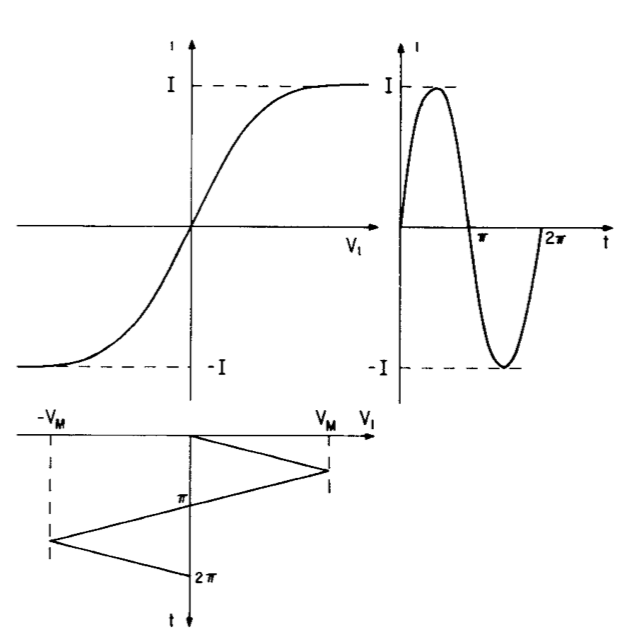
\includegraphics[width=1\textwidth]{Imagenes_Ej3/func.png}
	\caption{Transferencias etapa de conversion}
	\label{fig:linealizacion}
\end{figure}

Cuando se aplica una onda triangular de amplitud apropiada la transferencia del par diferencial redondea y achata las curvas de salida de la señal. Los dos resistores variables sirven para controlar la transferencia con tal de lograr una mejor forma en la onda. 

\subsection{Calibración}

En total, el circuito posee 4 potenciómetros que deben ajustarse para calibrar correctamente el VCO:


\begin{itemize}
\item La resistencia de realimentación del Schmitt trigger debe ajustarse para lograr el nivel de tension deseado, dados los componentes elegidos. Para eso se ponen 0 Volts a la entrada y se ajusta el preset hasta lograr una señal de $1kHz$.
\item El preset entre los emisores de los trasnsitores en el par diferencial debe ajustarse para lograr mejor simetría en la onda senoidal.
\item El preset a la entrada del conversor se ajusta para suavizar la triangular y lograr una onda senoidal.
\item El preset a la salida del sistema se ajusta para lograr una señal de 1 $Volt$ de amplitud. 
\end{itemize}


\subsection{Resultados Experimentales}
\subsubsection{Sumador}
En un principio se analizó como se comporta la etapa de transformación lineal del circuito. Para eso se lo estimuló con una señal continua de 0 a 5 Volts. En la siguiente imagen se muestra la transferencia de la etapa de transformación lineal, los puntos azules son los datos medidos mientras que la recta naranja representa la ecuación ideal:

\begin{figure}[H]	
	\centering
	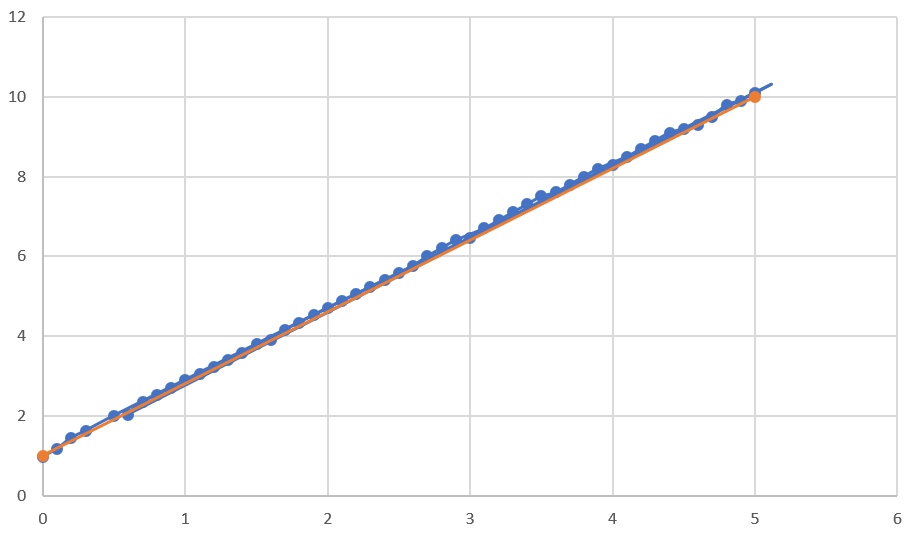
\includegraphics[width=1\textwidth]{Imagenes_Ej3/linealizacion.png}
	\caption{Transferencia primera etapa}
	\label{fig:linealizacion}
\end{figure}

El circuito cumple bien con la ecuación de la recta teórica a excepción del inicio, donde comienza aproximadamente 100 mV por encima del valor requerido.
\subsubsection{VCO}

Para Probar el VCO se lo estimuló nuevamente con una señal continua en el rango $0-5$ Volts, y en el modo estadítico del osciloscopio se esperaron al menos 2500 mediciones para tener un valor representativo de la desviación estándar de las mediciones. 

\begin{table}[H]
\centering
\begin{tabular}{lllll}\hline
Vin (V) &  Media (kHz) &  Mínima (kHz) &  Máxima (kHz) & Desviación Estándar (kHz) \\ \hline
0       & 1.12                   & 1.11                    & 1.14                    & $3X10^{-3}$                   \\
1       & 3.27                   & 3.26                    & 3.29                    & $8X10^{-3}$                         \\
2       & 5.26                   & 5.25                    & 5.27                    & $9X10^{-3}$                         \\
3       & 7.18                   & 7.14                    & 7.19                    & $1.1X10^{-2}$                         \\
4       & 9.01                   & 8.97                    & 9.05                    & $1.4X10^{-2}$                         \\
5       & 10.4                   & 10.39                   & 10.81                   & $1.9X10^{-2}$                        \\ \hline
\end{tabular}
\caption{Jitter etapa de conversion}
\end{table}

Salta a la vista que el valor de la desviación es varios ordenes de magnitud más pequeño que la media, entonces se habla de una baja dispersión de los datos, lo que significa una señal con bajo jitter. Además se ve que tanto la frecuencia a 0 Volts como la frecuencia a 5 Volts son mayores a las calculadas. A pesar de lo anterior, se cumple la relación lineal deseada entre la tensión de entrada y la frecuencia de salida del circuito. 

Por último se procedió a medir la distorsión armónica de la señal de salida con la función FFT del osciloscopio para corroborar que la forma sea la adecuada:

\begin{table}[H]
\centering
\begin{tabular}{ll}\hline
\multicolumn{1}{c}{Frecuencia fundamental (kHz)} & THD (\%) \\ \hline
1.1                                              & 0.51     \\
3.3                                              & 0.72     \\
5.29                                             & 1.442    \\
7.2                                              & 1.128    \\
9                                                & 1.376    \\
10.8                                             & 1.446   \\ \hline
\end{tabular}
\caption{Distorsion armónica}
\end{table}

En todos los casos la distorsión fue menor al 1,5\% pero se ve que es creciente respecto a la frecuencia. Si se calibrara el circuito para trabajar en cada frecuencia en específico, en vez de hacerlo una vez al principio se lograrían resultados mejores. En la siguiente imagen se observa la señal de salida, en los máximos y mínimos se ve una distorsion en la onda que ocaciona un aumento del THD:

\begin{figure}[H]	
	\centering
	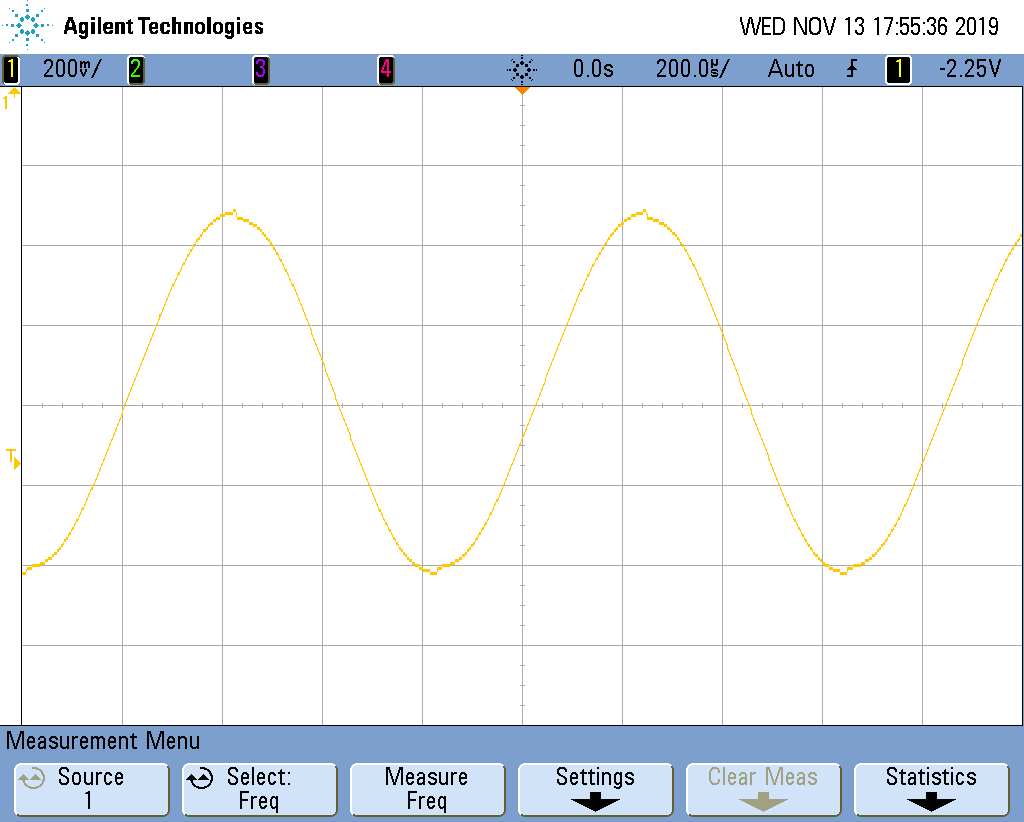
\includegraphics[width=1\textwidth]{Imagenes_Ej3/senoidal.png}
	\caption{Señal de salida}
	\label{fig:senoidal}
\end{figure}


\subsection{Conclusión}

En el presente ejercicio de logró diseñar e implementar un oscilador controlado por tensión para una entrada de 0 a 5 Volts y una frecuencia de salida de 1 a 10kHZ. Aunque los valores de tensiones y frecuencias no son exactamente los pedidos, están en el rango de error de calibración y tolerancia de los componentes. Se logró un THD menor al 1.5\% para todas las frecuencias, y un jitter relativamente bajo. No obstante, existen varias mejoras aplicables:


\begin{itemize}
\item Podría utilizarse un transistor tipo CMOS como switch en lugar de un BJT para lograr una menor distorsión y un tiempo  switch más rápido.
\item Para eliminar los armónicos en alta frecuencia puede agregarse algún tipo de filtro pasabajos.
\item Por último, agregar un filtro pasabanda con el Q adecuado puede ser una posibilidad para reducir el jitter en la señal.
\end{itemize}
